\documentclass[11pt]{article}
\usepackage[utf8]{inputenc}

\title{Astronomy 121: Analog Lab}
\author{Vikram Iyer}
\date{\today}
\usepackage{natbib}
\usepackage{graphicx}
\usepackage[margin=1.0in]{geometry}

\begin{document}

\maketitle

\begin{abstract}
  This lab experiment explores the basic principles of analog electronics for the purpose of processing RF signals and culminates in the design of an FM demodulator circuit as well as an amplifier that amplifies the demodulated input to a level sufficient to drive a speaker. The demodulator circuit uses an LC band pass filter centered below the dominant frequency of the carrier wave to produce an amplitude modulated signal.  This is followed by a diode detector used to remove the carrier frequency and obtain the original signal.  This demodulated signal is then input to a two stage biopolar amplifier composed of a common emitter gain stage and a low output impedance emitter follower stage used to drive a speaker. The effects of Johnson-Nyquist noise on this system were also studied and estimated to be on the order of .
  %INSERT JOHNSON NYQUIST NOISE NUMBER 
\end{abstract}

\section{Introduction}
  Analog circuits design is an integral part of systems involving radio frequencies including applications beyond communications such as radio-astronomy. While many signal processing tasks can be effectively implemented digitally, the reception and transmission of high frequency signals requires analog circuits.  This lab begins by exploring the basic circuit elements such as voltage dividers, passive filters, and diodes. After applying these concepts to design an FM demodulator circuit, we then explored the properties of bipolar transistors with the goal of designing an amplifier to play the demodulated FM signals through a speaker. Lastly we investigated the Johnson-Nyquist noise inherent to electric circuits and their effects on our FM radio system.

\section{Methods}
  \subsection{Voltage Division \& Filters}
      The voltage divider is a simple linear circuit which, as the name suggests, produces an output voltage $V_{out}$ that is a fraction of the original input voltage $V_{in}$.  
    \begin{figure}[h!]
    \centering
    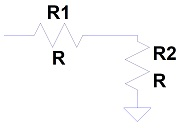
\includegraphics[scale=1.7]{voltage_divider.jpg}
    \caption{A resistive voltage divider.}
    \label{fig:voltage_divider}
    \end{figure}
    
    Figure ~\ref{fig:voltage_divider} above shows a resistive voltage divider.  We an analyze the output using Kirchoff's Current law to determine the voltage at the output:
    $$\frac{V_{out} - V_{in}}{R_1} + \frac{V_{out} - 0}{R_2}$$
    $$V_{out}\left(\frac{1}{R_1} + \frac{1}{R_2}\right) = \frac{V_{in}}{R_1}$$  
    $$V_{out}\left(\frac{R_1 + R_2}{R_1R_2}\right) = \frac{V_{in}}{R_1}$$  
    $$V_{out}= \left(\frac{R_2}{R_1+R_2}\right)$$  
    This result was tested using an Agilent 34405A Digital Multimeter to probe between the output and ground of a voltage divider constructed with two 1k$\Omega$ resistors with 5\% tolerance using an input of +5V DC from an Agilent E3631A Power Supply. The current through each resistor was then measured by connecting the multimeter in series with each resistor as well. After testing DC voltages a 1$V_{pp}$ 1MHz sine wave was applied to the circuit from an Agilent 33522A Arbitrary Waveform Generator and measured on an Agilent Infiniivision MS-S2014A Mixed Signal Oscilloscope.  After testing an individual voltage divider, a second divider was cascaded and tested with the same DC input.
    
    % TODO: insert oppenheim reference
    The same principles behind the voltage divider can be applied to analyze other passive circuit elements such as inductors and capacitors. In the case of these components, by applying the Laplace transform to their current and voltage relationships can be used to derive their impedance. The analysis of the voltage divider in terms of a generic complex impedance is algebraically the same, however because the impedance of inductors and capacitors are dependent on $\omega$, these circuits will exhibit different behaviors depending on the frequency of the input.
    The same equipment was used to test a voltage divider with two 1$\mu$F capacitors, and then the same configuration with a resistor from the output to ground.
    
    These principles can be used to design filters, circuits with frequency dependent characteristics which can be used to attenuate or amplify sinusoidal inputs of particular frequencies.  Filters are extremely useful in sensor applications as they can be used to remove unwanted noise at particular frequencies such as the 60Hz noise from AC power lines.
    An RC filter consisting of a single resistor and capacitor with the cutoff frequency (-3dB attenuation) at 100kHz can be designed as follows:
    \begin{figure}[h!]
    \centering
    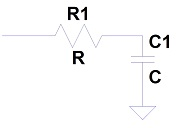
\includegraphics[scale=1.7]{lowpass.jpg}
    \caption{A first order RC low pass filter.}
    \label{fig:lowpass}
    \end{figure}
    
    $$\omega_c = 2\pi (100 kHz) = 2\pi \times 10^5  \frac{rad}{s}$$
    $$\omega_c = \frac{1}{R_1C_1}$$
    Choosing $C = 0.01\mu F$ we can determine an appropriate resistor value. 
    $$2\pi \times 10^5 = \frac{1}{R_1C_1}$$
    $$R_1 = \frac{1}{2\pi \times 10^{-3}}\approx 160\Omega$$
    
    \begin{figure}[h!]
    \centering
    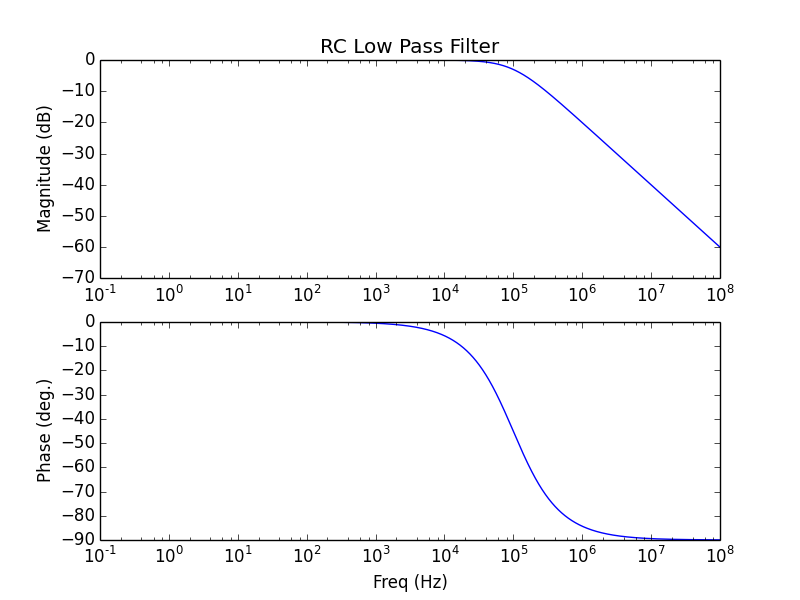
\includegraphics[scale=0.5]{rc_low_pass.png}
    \caption{Bode plot of a first order RC low pass filter showing the circuit's response to varying frequency.}
    \label{fig:lowpass_bode}
    \end{figure}
    
    Switching the order of the components changes this circuit to a high pass filter at the same cutoff frequency:
    
    \begin{figure}[h!]
    \centering
    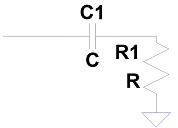
\includegraphics[scale=1.7]{highpass.jpg}
    \caption{A first order RC high pass filter.}
    \label{fig:highpass}
    \end{figure}
    
    If the same values are used then the RC time constant and therefore $f_c$ remain unchanged. The behavior of the filter in ~\ref{fig:lowpass} can be easily explained by the fact that a capacitor acts as a short circuit at high frequencies, creating a direct connection to ground and thereby diverting high frequency signals from the output. This circuit can be easily converted to a high pass filter by simply switching the two components. Intuitively this makes sense considering the capacitor, which acts as an open circuit at low frequencies, is now directly in the signal path.
    
    \begin{figure}[h!]
    \centering
    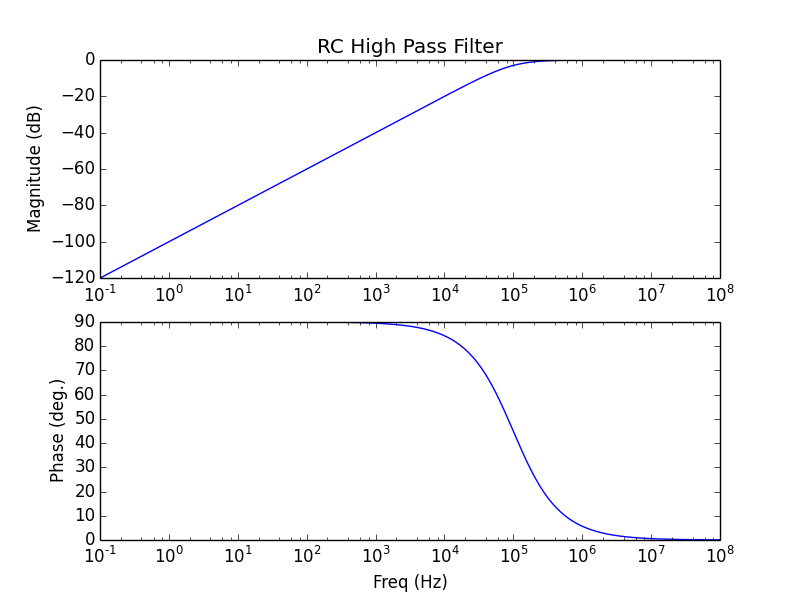
\includegraphics[scale=0.5]{rc_high_pass.png}
    \caption{Bode plot of a first order RC high pass filter showing the circuit's response to varying frequency.}
    \label{fig:highpass_bode}
    \end{figure}
    
    
    Inductors can also be combined with resistors and capacitors to create additional filter topologies. Below are band pass and band reject filters, which as the name suggests affect frequencies within a certain range.
    \begin{figure}[h!]
    \centering
    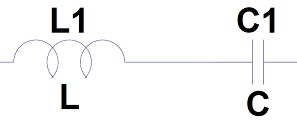
\includegraphics[scale=1.3]{lc_series.jpg}
    \caption{A band reject filter composed an inductor and a capacitor in series.}
    \label{fig:lc_series}
    \end{figure}
    
    Applying the Laplace transform yields the following expression for the impedance of a series LC circuit:
    $$Z = \frac{1}{j\omega C} + j\omega L $$
    $$Z = \frac{1}{j\omega C} + j\omega L \left(\frac{j\omega C}{j\omega C}\right)$$
    $$Z = \frac{j\omega^2 LC-j}{\omega C} $$
    
    \begin{figure}[h!]
    \centering
    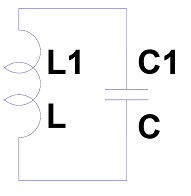
\includegraphics[scale=1.7]{lc_parallel.jpg}
    \caption{A band-pass filter composed an inductor and a capacitor in series.}
    \label{fig:lc_parallel}
    \end{figure}
    
    $$Z = \left(\frac{1}{j\omega L} + j\omega C\right)^{-1}$$
    $$Z = \left(\frac{1}{j\omega L} + j\omega C \left(\frac{j\omega L}{j\omega L}\right)\right)^{-1}$$
    $$Z = \left(\frac{j\omega^2 LC-j}{\omega C}\right)^{-1}$$
    
    
  \subsection{Diodes}
  In addition to resistors and capacitors semiconductor devices are also commonly used in circuits. Diodes are semiconductor devices that only allow current flow in one direction.  A silicon diode such as the 1N3597 used is formed by a junction of P and N type silicon.  Within a few micrometers of the actual interface, both sides are depleted of charge carriers. The net electric field creates a "built in potential" across this region that opposes the flow of charge from the P side to the N side of the diode without the application of an external voltage. Above this "turn on" voltage, the current allowed to pass through the diode increases exponentially with some dependence on temperature:
  $$ I = I_s^{\frac{ V_{BE} }{ V_{T} }}$$
  
  In order to test the properties of the 1N3597 diode, the Agilent test equipment previously mentioned was used to apply a DC voltage to the P terminal of the diode and the current through a 1k$\Omega$ resistor placed in series with the diode was measured. A 1$Vpp$ 1kHz sinusoid was also tested for comparison. 
  
  
  \subsection{FM Demodulation}
  A common mode of transmitting radio signals is through frequency modulation (FM). As the name suggests, this method involves encoding information as changes in frequency.  The primary advantage to this modulation scheme over amplitude modulation (AM) methods is its superior signal to noise ratio (SNR) when the signal level is above the noise floor. This makes intuitive sense as the amplitude of a signal can easily be affected by various sources of noise in every part of the signal path, however the frequency typically does not suffer from the same issues.
  In order to recover the original information from the raw FM signal such that it can be played through a speaker, we must demodulate it appropriately.  To do so we used the various circuit elements detailed above to first convert the changes in frequency to an amplitude modulated carrier wave, and then removed the carrier frequency to obtain the original input signal.
  
  \subsection{Transmission Lines \& Impedance Matching}
  High frequency signals such as received FM signals from an antenna can easily be affected by the cables through which they are transmitted and their interconnections.  In order to understand and demonstrate the effects of mismatched impedance at the ends of transmission lines we first observed the effects of physical "impedance mismatches" on manual impulses applied to cables of different thicknesses.  In order to understand the effects of different "impedance" values we tied cables of differing thicknesses together with one end attached to a stationary object, while another was held by hand.  By doing so with a piece of rope and an extension cord, we were able to observe the effects of the "transmission line" on an impulse applied to the cable.
  After testing physical disturbances along lengths of cable we performed similar tests with electrical signals to develop a more realistic understanding of the effects of interfaces along our signal path from our FM input received through the antenna all the way to the speaker output.  A 1MHz square wave was applied to an 16 ft cable connected to an oscilloscope.  The same input was tested with both 10$\Omega$ and 50$\Omega$ termination.
  
  \subsection{Bipolar Amplifiers}
  The previous sections addressed the issues of receiving, demodulating, and transmitting a signal through a cable; however oftentimes the amplitude of the demodulated output is far too low for the desired application. In the example of FM radio with the goal of driving a speaker, applying the raw output of the demodulator will not produce a sound from a speaker. In order to address this, we built an amplifier circuit using bipolar transistors to be able to play the signal from a speaker.
  The underlying physics of a bipolar junction transistors is similar to that of a PN junction diode. These devices are formed using two PN interfaces.  These devices are named accordingly as either NPN or PNP.  When the base-emitter junction in an NPN transistor is forward biased with an appropriate voltage, a small current of holes flows from the base to the emitter while a much larger number of electrons flows into the base.  Because of the very thin base width, the large flow of electrons is swept into the collector producing a positive current flow from the collector to the emitter. It is this current amplification property of a transistor (small base current producing a large collector current) that allows us to use transistors to build amplifiers.
  When designing the amplifier circuit, we first ensured that the devices were operating in the appropriate region (forward active).  For bipolar transistors, this required accounting for the nonlinear relationship between base emitter voltage and collector current in order to appropriately bias the device.  After biasing the device, we approximated the behavior of the amplifier with a linear model for small signals in order to determine the IO impedances as well as the amplification.
  %TODO cite Razavi
  
  \subsection{Noise Figures}
  As previously explained the models we used to design our amplifiers were approximations of the devices' actual behavior and assumed ideal conditions. While these simplified models function relatively well in practice and are useful for analyzing complex circuits, the measured output of real circuits can be affected by other factors.  One such factor is Johnson-Nyquist noise.  Going back to the context of FM radio, noise can be interpreted literally as unwanted sound.  Johnson-Nyquist or thermal noise arises as a result of the random movement of charge carriers within materials due to thermal energy. In any material at a temperature above absolute zero, there is some motion of particles.  The relationship between temperature and noise is shown below:
  $$P_sig = 4k_BTBR$$
  We attempted to obtain a measurement of thermal noise from a 50$\Omega$ resistor.  Because the very low amplitude of the noise, we first headed the resistor by applying 10V and therefore dissipated a total of 2W across the resistor.  This caused the resistor to increase significantly in temperature, at which point we measured the amplified voltage output using an AC1068 amplifier and attempted to determine the standard deviation from the expected voltage by viewing the resulting waveform on a Tektronix TDS350 200MHz oscilloscope.
  
  \subsection{Central Limit Theorem}
  To gain a better conceptual understanding of the mathematics underlying the Johnson-Nyquist noise we observed, we wrote a python script to demonstrate the central limit theorem.

\section{Results \& Discussion}
  \subsection{Voltage Division \& Filters}
  We measured the voltage under different conditions as explained.  The results are shown below.
  For a +5V DC input:
  $$V_{out} =  2.494 V$$
  $$I_{R1} = 2.51 mA$$
  $$I_{R1} = 2.49 mA$$
  
  For a 1MHz $200mV_{pp}$ sine wave input:
  $$V_{out} = 114mVpp out$$
  
  The measured values are close to the calculated ratio of $\frac{1}{2}$, and the slight variations are likely due to small mismatches in resistance.  In this case we chose to use 1k$\Omega$ resistors in part because they were readily available, however when choosing between high and low impedance values for a voltage divider with the same ratios, the current flowing through each branch should be considered. Larger values should be preferred in most cases to minimize the power loss in these resistors as for a given voltage, the power consumed by the circuit is inversely proportional to the resistance:
  $$P = IV = \frac{V^2}{R}$$ 
  
  We also tested cascaded voltage dividers.
  For a +5V DC input:
  $$V_{out1} =  2 V$$
  $$V_{out2} =  1 V$$
  
  For a 1MHz $200mV_{pp}$ sine wave input:
  $$V_{out1} = 93 mV_{pp}$$
  $$V_{out2} = 50 mV_{pp}$$
  
  When cascading voltage dividers, each block can be abstracted away as an equivalent resistance looking back to the output of the previous stage.  This equivalent resistance is known as the Thevenin resistance of the circuit and in this case is placed in parallel with the resistor in the voltage divider.  This added resistance changes the voltage division at each stage.
  
  After measuring the output of the resistive voltage dividers we tested voltage dividers using capacitors.
  For a 1MHz $200mV_{pp}$ sine wave input:
  $$V_{out} = 30 mVpp$$
  This may not have been an accurate measurement as the output on the scope had a frequency of 1MHz, it was heavily distorted. Additionally the capacitive voltage divider had no effect on the DC value of the signal.
  
  The same measurement was performed after placing a 1k$\Omega$ resistor from the output to ground.  There was no measurable output on the oscilloscope for this circuit.  The reason for the sharper attenuation of the second circuit can be seen by analyzing its impedance.  We can first find the expression for the parallel combination of the resistor and capacitor, and then substitute this into the voltage divider equation:
  $$Z_2 = \left(j\omega C + \frac{1}{R}\right)^{-1}$$
  $$Z_2 = \frac{R}{j\omega RC + 1}$$
  $$\frac{Z_2}{Z_1 + Z_2} = \frac{\frac{R}{j\omega RC + 1}}{\frac{1}{j\omega C} + \frac{R}{j\omega RC + 1}}$$
  
  Simplifying this expression yields a two poles in the denominator, which will therefore cause -40dB/dec attenuation above the second pole. This measurement and calculation shows that faster attenuation can be achieved by increasing the order of the filter. In general this can be achieved by cascading filters or modifying them as shown in this example.  In the case of cascaded filters, by properties of the Laplace transform we can see that the frequency responses of the filters will be multiplied. Although higher order filters can be used to achieve sharper attenuation of unwanted signals, one must be careful to design the pass bands of filters such that signals of interest will not be unintentionally attenuated. 
  % TODO: Cite Oppenheim
  
  \subsection{Diodes}
  We applied various voltages to the diode to determine the point at which it would begin allowing current to flow.  We found that the diode allows current to flow freely at voltages around or above 0.7V.  Measurements of voltage and current flowing through a 1k$\omega$ resistor attached in series are shown.
  
    \begin{figure}[h!]
    \centering
    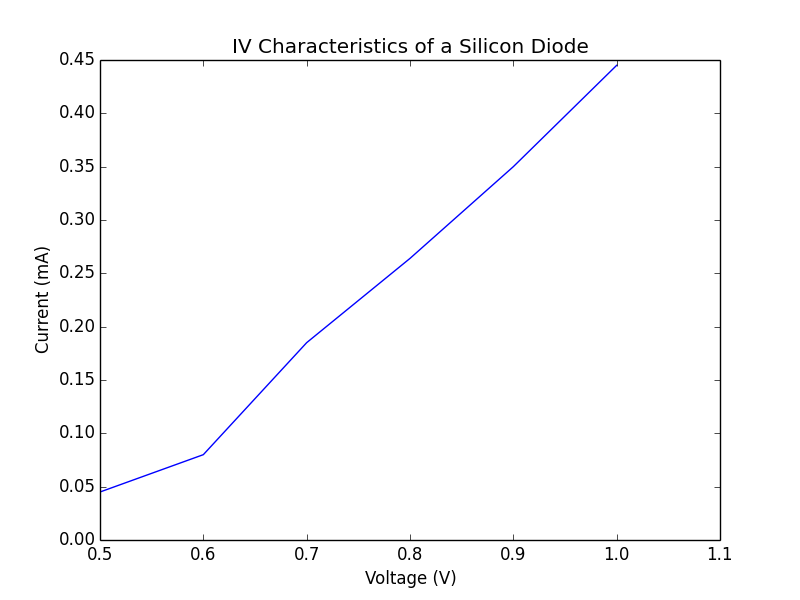
\includegraphics[scale=0.5]{diode_iv.png}
    \caption{This plot shows the effect on the current passing through a silicon diode in response to an increasing voltage applied across it.}
    \label{fig:diode_iv}
    \end{figure}
    
  Even from the limited set of measurements shown, the region of the graph from 0.5 to 0.7V shows a roughly exponential increase. A more precise characterization of the device could be obtained using a semiconductor parameter analyzer, however this data is enough to show the known mathematical relationship can be observed in practice.     
  
  After investigating the current and voltage relationship of the diode we applied a 1kHz $1V_{pp}$ sinusoid with 0.7V DC offset and measured the output on an oscilloscope.  The resulting waveform was simply the original waveform with all of the negative peaks subtracted. This makes sense considering the characteristics of the diode shown in ~\ref{fig:diode_iv}.
  The output of the diode was then applied to a first order RC low pass filter as illustrated in ~\ref{fig:lowpass} with a cutoff frequency of 1kHz. The resulting signal was simply a DC value corresponding to the amplitude of the original input. This output shows that the combination of a diode and low pass filter can be used to detect only the amplitude of a signal, a property that can be used to demodulate AM signals. This makes sense intuitively as after the diode rectifies the signal, a low pass filter will smooth the signal to eliminate the high frequency components resulting from the removal of half of the waveform.
  
  \subsection{FM Demodulation}
  As explained previously, the information in the received FM signal is represented by changes in frequency. The full circuit diagram for the FM demodulator is shown below.
    \begin{figure}[h!]
    \centering
    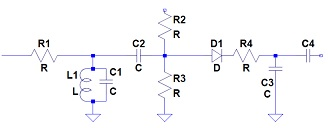
\includegraphics[scale=1.7]{demodulator.jpg}
    \caption{A full circuit diagram of the FM demodulator.}
    \label{fig:demodulator}
    \end{figure}
    
  In order to demodulate the signal we first applied an LC band pass filter with a cutoff frequency 1MHz, slightly below the frequency of the FM carrier wave which was at 1.045MHz.  The same methods used to analyze the parallel LC circuit shown in ~\ref{fig:lc_parallel} can be used to determine the components that should be used for this filter:
  
  $$1MHz = 2\pi \times 10^6 = \frac{1}{\sqrt{LC}}$$
  
  Choosing C to be 0.01$\mu F$ and a value for L close to 2.533$\mu H$ will produce the appropriate filter. Because the resonance peak of the circuit is at 1MHz, the FM input signal will fall in the roughly linear region above it therefore translating changes in frequency the corresponding amounts of attenuation to a change in the amplitude of the signal.  As shown by the investigation of the diode detector circuit, the combination of the diode followed by a low pass filter will detect the envelope of the signal corresponding to the varying amplitude. To center the low pass filter appropriately to eliminate the 1.045MHz carrier frequency, we can use the values C=1nF and R = $150\Omega$.
  Before passing the input through the diode detector, we must ensure that the diode is appropriately biased at a value in the range of 0.6 to 0.8V as shown.  This can be accomplished using the resistive divider shown in ~\ref{fig:demodulator}.  Using a 1V DC input we can determine the resistor values by applying the voltage divider equation and choosing the value of $R_2$ to be 1k$\Omega$:
  $$0.7 = \frac{1000}{1000 + R_1}$$
  $$0.7R_1 = 300$$ 
  $$R_1 = 428.5\Omega \approx 400\Omega$$
  
  In addition to biasing the diode appropriately, we placed capacitors between each stage of the circuit in order to isolate the AC small signals of interest.  The combination of C2 followed by the resistive divider essentially centers the AC input about a DC offset voltage determined by the resistive divider that in this case will allow the diode to function appropriately.  We took a similar approach for biasing the transistors, which is the reason for placing the additional capacitor C4 at the end of the demodulation circuit.
  
  \subsection{Transmission Lines \& Impedance Matching}
  Prior to testing cables with electrical signals, we applied physical waves to cables of different thicknesses. We began by observing an extension cord attached to a solid object, which cased an inverted reflection of the signal.  Next we observed the effects of leaving the cable loosely tied to a stationary object with a thinner cord.  We tried different combinations of cables tied tightly and loosely to solid objects and determined that adjusting the tightness of the cords allowed us to control the amount to which the input was reflected back.
  When trying a similar experiment using a 16ft coax cable with a 1MHz input as previously described, we were able to clearly observe the effects of the reflected signal on an oscilloscope after increasing the length of the cable beyond 8 ft.  The distortion in the measured waveform was manifested as what appeared to be a delay by 44ns part way through the rising edge of the square wave.  Based on these measurements the pulse appeared to be traveling at a speed of 0.363 ft/ns.
  \subsection{Bipolar Amplifiers}
  In order to amplify our input signal we used a common emitter amplifier to produce a large gain.  We degenerated the transistor with a resistor from the emitter to ground.  Although this configuration reduces gain, it allows us to better predict the behavior of the transistor by decreasing the dependence of the gain on the properties of the device (which are in many cases imprecise). Additionally, placing a capacitor in parallel with this resistor causes the gain of the amplifier to become frequency dependent. 
  
    \begin{figure}[h!]
    \centering
    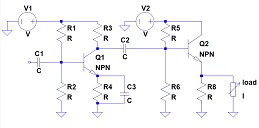
\includegraphics[scale=1.7]{amplifier.jpg}
    \caption{Circuit diagram of the two stage amplifier consisting of a common emitter cascaded with an emitter follower.}
    \label{fig:amplifier}
    \end{figure}
  
  The circuit can be analyzed as follows.  We begin by choosing a value for the collector current to be 1mA so that we can proceed with the small signal analysis:
  $$g_m = \frac{I_c}{V_T} = \frac{1}{26} = 0.0385$$
  $$A_v = -\frac{cg_m R_c}{g_m R_E + 1} = 2$$
  Choosing the value of $R_C$ to be 1k:
  $$A_v = -\frac{38.5}{0.0385R_E + 1} = 2$$
  Solving for $R_E$ yields a value of $525.9\Omega \approx 500 \Omega$.  Proceeding with this value of $500\Omega$, we can then determine the amount of attenuation required to produce a gain of 10 at 10kHz.
  $$A_v = -\frac{38.5}{0.0385(500)x + 1} = 10$$
  An attenuation factor of 0.25 will produce a gain of 10 at 10kHz.  In order to achieve this we need an attenuation of at least $20log(0.25) = -12$ for frequencies above 10kHz.  If we select the capacitor to place the -3dB point at 5kHz, with a -20dB/dec slope this should satisfy this requirement.  The impedance can therefore be analyzed as follows:
  $$Z_E = \left(\frac{1}{R_E}+j\omega C\right)^{-1}$$
  $$Z_E = \frac{R_E}{j\omega R_E C + 1}$$
  $$\frac{1}{R_E C} = 2\pi 5\times 10^3$$
  $$\frac{1}{C} = 1000\pi 5\times 10^3$$
  $$C = 0.06366\mu F$$
 
  In order to achieve a current of 1mA using we must set $V_BE$ to bias the transistor appropriately:
  $$V_E = (1mA)(500\Omega) = 0.5V$$
  We assumed that $I_S$ for the device, which was not given), to be at least an order of magnitude smaller than the chosen $I_C$ of 1mA.
  
  $$V_BE = V_T ln(\frac{1}{10}) \approx 0.6$$
  
  To set the base voltage appropriately we used a resistive voltage divider to reduce the 1V input.  Choosing $R_2$ to be 1$k\Omega$ we determined $R_1$ to be 315$\Omega$.
  $$1 = \frac{1000}{1000 + R_1}$$
  After determining all of the resistances we calculated the input and output impedances of the amplifier.
  To determine the input resistance, we can "look into" the base. The small signal resistance will be $r_{\pi}=\frac{\beta}{g_m}$.  For a typical $\beta = 100$, $r_{\pi} = 3.33k\Omega$. We assumed for all of the previous calculations that the early voltage $V_A=\inf$, therefore the output impedance is simply $R_C=1k\Omega$.  In practice $V_A$ is not infinite, however for most BJTs this value is large enough such that the resistance due to Early Voltage will have little effect on the output impedance when placed in parallel with the chosen $R_C$.
  If additional information about the capacitances at the emitter and collector were provided the bandwidth of the amplifer could have been determined as well. Assuming these values are on the order of a few pF, as is typical for most BJTs, we can rougly approximate the order of magnitude of the poles that will limit the bandwidth of the amplifier.
  $$\frac{1}{RC}=\frac{1}{10^3 10^-12}= 2\pi 10^9 Hz$$
  The bandwidth of the amplifier was therefore clearly well above the range of audible frequencies.
  Although the required gain could be easily met with a single stage amplifier, in order to drive the speaker we created a separate output stage.  For the first stage of this amplifier we chose a common emitter topology which can be designed to have a large gain as shown.  The common emitter amplifier suffers from an output impedance significantly higher than that of an 8$\Omega$ speaker.  In order to address this impedance matching issue and provide the appropriate amount of current at the output required to drive the speaker we then cascaded the common emitter amplifier with a voltage follower circuit. 
  The emitter follower amplifier was designed by biasing the transistor at approximately 2.5V which ensures that even a signal with a 1V swing will keep the base voltage above the approximately 0.7V required to keep BJTs operate in the forward active region. We chose the emitter resistance to be small $R_E = 10$ such that we could attempt to match the 8$\Omega$ load and provide maximum power transfer.
  
  \subsection{Noise Figures}
  When trying to approximate the Johnson-Nyquist noise we began by measuring the temperature of the resistor.  When dissipating 2W the resistor was 183 $^{\circ}$C.
  This value differs greatly from the value predicted by the Stefan-Boltzman law, however it was very difficult to use this property to verify the measurement without any knowledge of the resistor itself or its properties.
  $$A = h\pi d + 2\pi r^2$$
  $$A = (0.016)(0.0045\pi)+2\pi \frac{0.0045}{2}^2 \approx 0.00341$$
  $$P = \left( \frac{2}{0.00341}(1)(5.67) \right)^{\frac{1}{4}}$$
  The measured value of temperature appeared to be accurate considering even after allowing the resistor to cool down for a few minutes after switching off the power supply it remained warm to the touch.
  Attempting to measure the noise in this resistor was equally difficult.
  We estimated the amplitude of the noise as follows:
  $$\sqrt{v^2_n} = \sqrt{(4)(1.38\times 10^{-23}(459)(50)} = 1.123 nV/\sqrt{Hz}$$
  For a 10MHz input this corresponds to an amplitude of 3.551 $\mu V$.  In order to 
  amplify these signals appropriately we needed:
  $$20 log(\frac{0.000351}{1}) \approx 70 dB$$
  In order to achieve a gain of 70 dB we cascaded multiple amplifiers.
  The noise figure we calculated based on these values was on the order of 21.16 $\mu$V.  As explained it was very difficult to determine this value accurately and the variance of our values on an mV scale was 132mV. This clearly shows that our attempt to measure the noise in the circuit was highly inaccurate; however, based on the theoretical calculations of Johnsons-Nyquist noise at room temperature, for the signals we were using the noise would have been in the nV range and therefore negligible compared to our actual input signal.
  
  \subsection{Central Limit Theorem}
  The program central\_limit.py demonstrated the central limit theorem by repeatedly sampling a Poisson distribution and showing that the means of the samples approach a normal distribution. 
  
    \begin{figure}[h!]
    \centering
    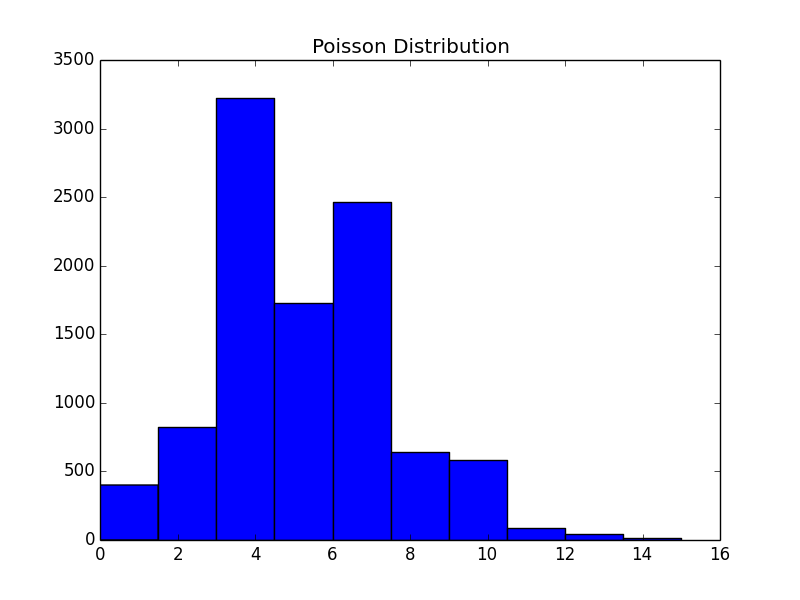
\includegraphics[scale=0.4]{poisson.png}
    \caption{Original Poisson distribution.}
    \label{fig:poisson}
    \end{figure}
    
    \begin{figure}[h!]
    \centering
    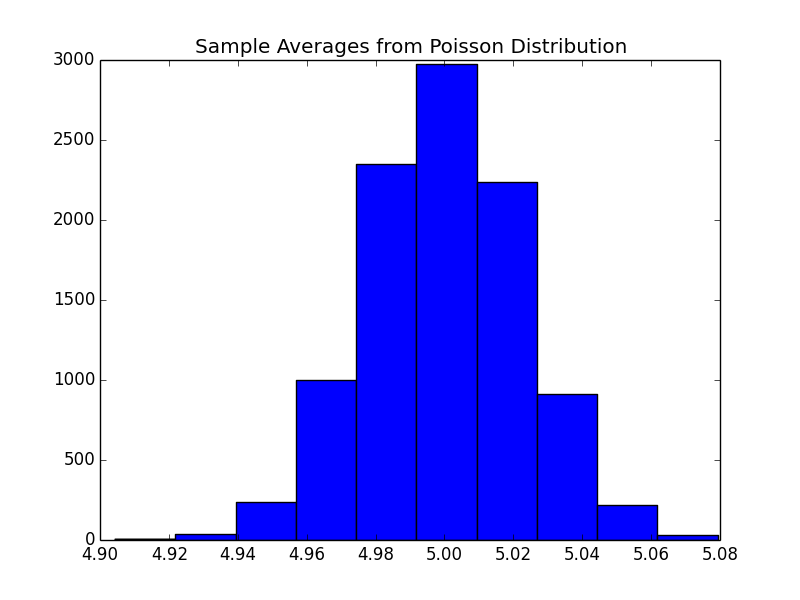
\includegraphics[scale=0.4]{normal.png}
    \caption{Plot of 10000 sample averages from the original distribution.}
    \label{fig:normal}
    \end{figure}
    
  The source code for generating these figures is available at https://github.com/viyer/astro121  

\section{Conclusion}
  This series of lab experiments developed both a conceptual and practical understanding of analog electronic systems and culminated in the design of functional circuits with important applications for radio communications. The demodulation of FM was a good example of both the mathematics of the signal processing challenges associated with the task as well as the practical aspect of amplifying the final output to a useful amplitude. Perhaps the most important practical aspect of the lab was the intuition and understanding developed about noise. Noise is present in all electronic systems and oftentimes the signal processing techniques and the circuits or algorithms used implement them are designed to eliminate noise and ensure that the system can produce the desired data. Understanding the process of circuit design to address these trade offs and the their causes was a valuable learning experience.
\end{document}
